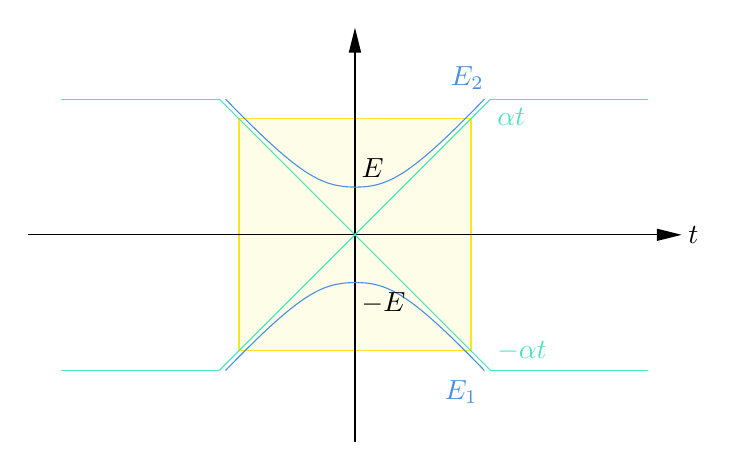
\begin{tikzpicture}[x=0.75pt,y=0.75pt,yscale=-1,xscale=1]
    %uncomment if require: \path (0,300); %set diagram left start at 0, and has height of 300
    
    %Shape: Square [id:dp8316656627568306] 
    \draw  [color={rgb, 255:red, 248; green, 231; blue, 28 }  ,draw opacity=1 ][fill={rgb, 255:red, 248; green, 231; blue, 28 }  ,fill opacity=0.1 ] (243.53,93.66) -- (355.31,93.66) -- (355.31,205.44) -- (243.53,205.44) -- cycle ;
    %Straight Lines [id:da5262129730259233] 
    \draw    (142,149.55) -- (454.83,149.55) ;
    \draw [shift={(456.83,149.55)}, rotate = 180] [fill={rgb, 255:red, 0; green, 0; blue, 0 }  ][line width=0.08]  [draw opacity=0] (12,-3) -- (0,0) -- (12,3) -- cycle    ;
    %Straight Lines [id:da9470135996804132] 
    \draw    (299.42,249.3) -- (299.42,51.81) ;
    \draw [shift={(299.42,49.81)}, rotate = 90] [fill={rgb, 255:red, 0; green, 0; blue, 0 }  ][line width=0.08]  [draw opacity=0] (12,-3) -- (0,0) -- (12,3) -- cycle    ;
    %Straight Lines [id:da5726298035471948] 
    \draw [color={rgb, 255:red, 80; green, 227; blue, 194 }  ,draw opacity=1 ]   (234.05,84.19) -- (364.78,214.92) ;
    %Straight Lines [id:da5750691866909603] 
    \draw [color={rgb, 255:red, 80; green, 227; blue, 194 }  ,draw opacity=1 ]   (234.05,214.92) -- (364.78,84.19) ;
    %Straight Lines [id:da33156968789479] 
    \draw [color={rgb, 255:red, 80; green, 227; blue, 194 }  ,draw opacity=1 ]   (364.78,84.19) -- (440.83,84.19) ;
    %Straight Lines [id:da25720871020587444] 
    \draw [color={rgb, 255:red, 80; green, 227; blue, 194 }  ,draw opacity=1 ]   (364.78,214.92) -- (440.83,214.92) ;
    %Straight Lines [id:da3245228029119711] 
    \draw [color={rgb, 255:red, 80; green, 227; blue, 194 }  ,draw opacity=1 ]   (158,84.19) -- (234.05,84.19) ;
    %Straight Lines [id:da37062892559863125] 
    \draw [color={rgb, 255:red, 80; green, 227; blue, 194 }  ,draw opacity=1 ]   (158,214.92) -- (234.05,214.92) ;
    %Curve Lines [id:da6363741925899513] 
    \draw [color={rgb, 255:red, 74; green, 144; blue, 226 }  ,draw opacity=1 ]   (237.05,84.19) .. controls (272.83,121.01) and (283.22,126.43) .. (299.42,126.55) .. controls (315.61,126.68) and (326.5,120.68) .. (361.78,84.19) ;
    %Curve Lines [id:da8947989113569657] 
    \draw [color={rgb, 255:red, 74; green, 144; blue, 226 }  ,draw opacity=1 ]   (237.05,214.92) .. controls (272.83,178.1) and (283.22,172.68) .. (299.42,172.55) .. controls (315.61,172.43) and (326.5,178.43) .. (361.78,214.92) ;
    
    % Text Node
    \draw (366.78,87.59) node [anchor=north west][inner sep=0.75pt]  [color={rgb, 255:red, 80; green, 227; blue, 194 }  ,opacity=1 ]  {$\alpha t$};
    % Text Node
    \draw (366.78,211.52) node [anchor=south west] [inner sep=0.75pt]  [color={rgb, 255:red, 80; green, 227; blue, 194 }  ,opacity=1 ]  {$-\alpha t$};
    % Text Node
    \draw (301.42,123.15) node [anchor=south west] [inner sep=0.75pt]    {$E$};
    % Text Node
    \draw (458.83,149.55) node [anchor=west] [inner sep=0.75pt]    {$t$};
    % Text Node
    \draw (362.78,80.79) node [anchor=south east] [inner sep=0.75pt]  [color={rgb, 255:red, 74; green, 144; blue, 226 }  ,opacity=1 ]  {$E_{2}$};
    % Text Node
    \draw (359.78,218.32) node [anchor=north east] [inner sep=0.75pt]  [color={rgb, 255:red, 74; green, 144; blue, 226 }  ,opacity=1 ]  {$E_{1}$};
    % Text Node
    \draw (301.42,175.95) node [anchor=north west][inner sep=0.75pt]    {$-E$};
    
    
    \end{tikzpicture}
    